%%
%% This is file `sample-sigconf.tex',
%% generated with the docstrip utility.
%%
%% The original source files were:
%%
%% samples.dtx  (with options: `sigconf')
%% 
%% IMPORTANT NOTICE:
%% 
%% For the copyright see the source file.
%% 
%% Any modified versions of this file must be renamed
%% with new filenames distinct from sample-sigconf.tex.
%% 
%% For distribution of the original source see the terms
%% for copying and modification in the file samples.dtx.
%% 
%% This generated file may be distributed as long as the
%% original source files, as listed above, are part of the
%% same distribution. (The sources need not necessarily be
%% in the same archive or directory.)
%%
%% The first command in your LaTeX source must be the \documentclass command.
\documentclass[sigconf, nonacm, natbib, screen, balance=False]{acmart}

% Documentation for packages
% - ACM Article Template
%    https://www.acm.org/publications/proceedings-template
% - Pseudocode typesetting CLRS-style:
%    https://www.cs.dartmouth.edu/~thc/clrscode/clrscode3e.pdf
% - Python code typesetting
%    http://ctan.uib.no/macros/latex/contrib/listings/listings.pdf
% - AMS Math
%    http://ctan.uib.no/macros/latex/required/amsmath/amsldoc.pdf
% - Graphics
%    http://ctan.uib.no/macros/latex/required/graphics/grfguide.pdf

\usepackage{clrscode3e}  
\usepackage{listings}
\lstset{language=Python, basicstyle=\ttfamily}

% based on https://tex.stackexchange.com/questions/279240/float-for-lstlisting
\usepackage{float}
\floatstyle{ruled}
\newfloat{listing}{tbph}{lop}
\floatname{listing}{Listing}
\def\lstfloatautorefname{Listing} % needed for hyperref/auroref

\citestyle{acmauthoryear}

%% end of the preamble, start of the body of the document source.
\begin{document}

%%
%% The "title" command has an optional parameter,
%% allowing the author to define a "short title" to be used in page headers.
\title{Replace by your report title}
\subtitle{INF221 Term Paper, NMBU, Autumn 2021}

\author{Jane Dane}
\email{jane.dane@nmbu.no}
\affiliation{}  % separates Jane's and Joe's author block

\author{Joe Doe}
\email{joe.doe@nmbu.no}

%% The abstract is a short summary of the work to be presented in the
%% article.
\begin{abstract}
  In this paper, we analyse \dots 
\end{abstract}


%%
%% This command processes the author and affiliation and title
%% information and builds the first part of the formatted document.
\maketitle

\section{Introduction}\label{sec:intro}

In this section, provide a brief introduction to the term paper's
topic and give an overview of the material that follows.

\section{Theory}\label{sec:theory}

Provide a brief description of the algorithms you will be
investigating, including pseudocode for the algorithms. Describe in
particular the expected runtime of algorithms in terms of problem
size.  Use a separate subsection for each algorithm.

\subsection{Algo 1}\label{sec:algo1}

\begin{listing}
  % Pseudocode caption above the code.
  \caption{Insertion sort algorithm from \citet[Ch.~2.1]{CLRS_2009}.}
  \label{lst:insertion_algo}
  %
  % For documentation on how to typeset CLRS-style pseudocode, see
  % https://www.cs.dartmouth.edu/~thc/clrscode/clrscode3e.pdf
  %
  \begin{codebox}
    \Procname{$\proc{Insertion-Sort}(A)$}
    \li \For $j \gets 2$ \To $\attrib{A}{length}$
    \li \Do
    $\id{key} \gets A[j]$
    \li     $i \gets j-1$
    \li      \While $i>0$ and $A[i] > \id{key}$
    \li      \Do
    $A[i+1] \gets A[i]$
    \li         $i \gets i-1$
    \End    
    \li       $A[i+1]\gets \id{key}$
    \End
  \end{codebox}
\end{listing}

Pseudocode for the first algorithm is shown in
Listing~\ref{lst:insertion_algo}. Best case runtime for this algorithm
is

\begin{equation}
  T(n) = \Theta(n) \;.  \label{eq:ins_sort_best}
\end{equation}

It is achieved for correctly sorted input data.

\subsection{Algo 2}\label{sec:algo2}

Lorem ipsum \dots


\section{Methods}\label{sec:methods}

In this section, you shall described how you performed the
benchmarks:
\begin{itemize}
\item What test-data did you use and how was it generated?
\item How did you execute your benchmarks?
\item How did you measure runtimes?
\item What kind of computer did you use, and what software versions?
\item Provide git hashes of all relevant files!
\item This section should be divided into several subsections.
\end{itemize}

\begin{listing}
  % Listing captions above the listing.   
  \caption{Draft benchmark setup.}
  \label{lst:bench_setup}
  \begin{lstlisting}
times = []
for k in range(1, 5):
   n = 2**k
   times.append(bench(func, n))
  \end{lstlisting}
\end{listing}

\begin{table}
  % Table captions always come *above* the table.
  \caption{Versions of files used for this report; GitLab repository
    \url{https://x.y.z}.}
  \label{tab:hashes}
  \begin{tabular}{ll}
    \hline
    File & Git hash \\\hline
    \verb!run_bench.ipynb! & \verb!42a44d2a6! \\
    \verb!results.pkl! & \verb!65342aed2! \\\hline
  \end{tabular}
\end{table}

\section{Results}\label{sec:results}

\begin{figure}
  \centering
  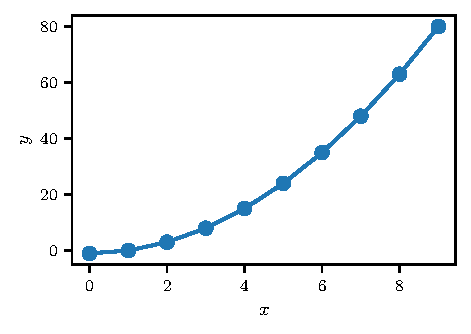
\includegraphics{sample_plot}
  % figure captions below figure
  \caption{Benchmark results for \dots.}
  \label{fig:bench}
\end{figure}

Here, you should present your results. Provide clear figures with tidy
lettering in legible font sizes. Figures should not be resized when
included, so prepare them for the column width of 84~mm. For good
quality, export figures as PDF files from Python.

The results section should be divided into several subsections.

\section{Discussion}\label{sec:discussion}

In this section, you should summarize your results and compare them to
expectations from theory presented in Sec.~\ref{sec:theory}.

% In the acks section, you can thank people for help.
\begin{acks}
We are grateful to \dots for \dots.
\end{acks}


%% The next two lines define the bibliography style to be used, and
%% the bibliography file.
\bibliographystyle{ACM-Reference-Format}
\bibliography{sample_bib}

\end{document}
